\documentclass{standalone}
\usepackage{tikz}
\usetikzlibrary{shapes.geometric, arrows}

\begin{document}

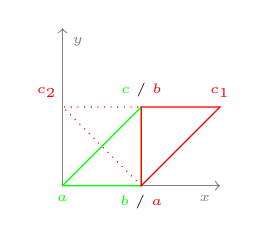
\begin{tikzpicture}

%draw the main coordinate system axes
\draw[->, gray] (0,0) -- (2,0) node[anchor=north east]{\tiny $x$};
\draw[->, gray] (0,0) -- (0,2) node[anchor=north west]{\tiny $y$};

\draw[green] (0,0) node[anchor=north] {\tiny $a$} -- (1,0) -- (1,1) -- cycle;
\draw[red] (1,0) node[anchor=north, green] {\tiny $b$ \color{black} / \color{red} $a$} -- (1,1) node[anchor=south, green] {\tiny $c$ \color{black} / \color{red} $b$} -- (2,1) node[anchor=south] {\tiny $c_1$} -- cycle;
\draw[red,dotted] (1,0) -- (0,1)  node[anchor=south,xshift=-0.2cm] {\tiny $c_2$} -- (1,1);

\end{tikzpicture}
\end{document}